\section{System design}

\subsection{Desired System Properties}

\begin{frame}{Desired System Properties}
    \begin{itemize}
        \item utilizes machine learning
        \item detects characteristic values
            \begin{itemize}
                \item fast (goal 100Hz)
                \item accurate
                \item independent of pose
            \end{itemize}
        \item non-obstructive
            \begin{itemize}
                \item flexible
                \item wireless
                \item light
            \end{itemize}
        \item software suitable for fast prototyping
        \item cheap
    \end{itemize}
\end{frame}

\subsection{Sensors}

\begin{frame}{Sensors}{Possible Choices}
    \begin{figure}
        \centering
        \begin{columns}[t]
            \column{.3\textwidth}
            \textbf{Flex sensors}
            \begin{minipage}[t][\textwidth][c]{\textwidth}
                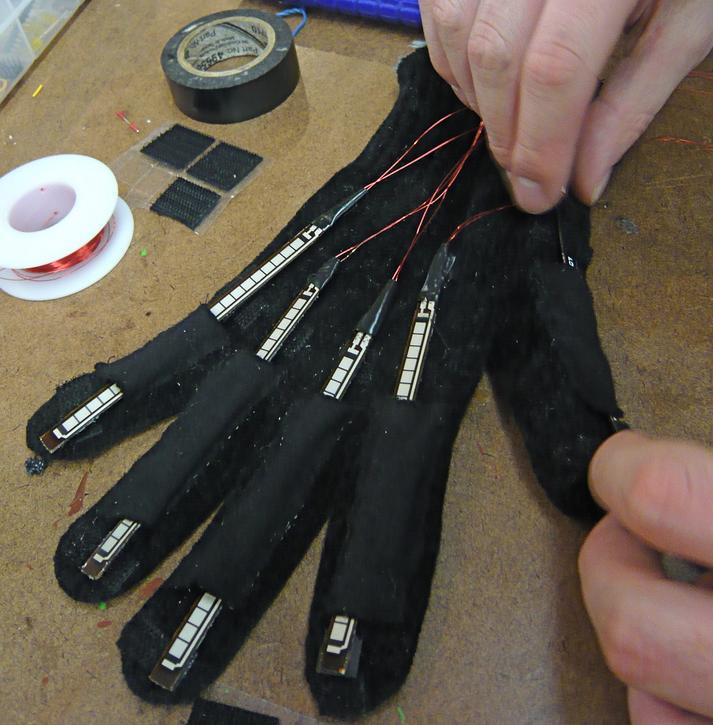
\includegraphics[width=\textwidth]{../common/images/flex-glove}
            \end{minipage}
            \imagesource{https://www.flickr.com/photos/indiamos/3060497602}

            \uncover<2->{
                \column{.3\textwidth}
                \textbf{Visual system}
                \begin{minipage}[t][\textwidth][c]{\textwidth}
                    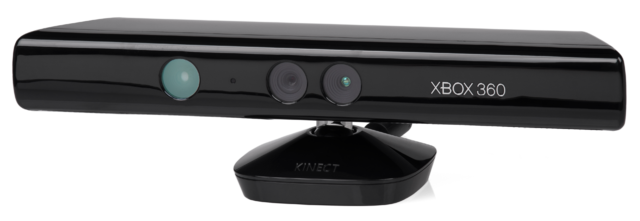
\includegraphics[width=\textwidth]{../common/images/kinect}
                \end{minipage}
                \imagesource{https://de.wikipedia.org/wiki/Kinect\#/media/File:Xbox-360-Kinect-Standalone.png}
            }

            \uncover<3->{
                \column{.3\textwidth}
                \textbf{IMUs}
                \begin{minipage}[t][\textwidth][c]{\textwidth}
                    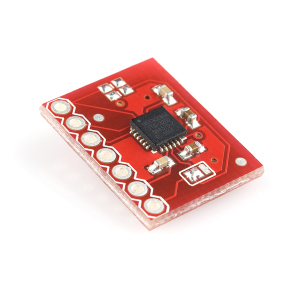
\includegraphics[width=\textwidth]{../common/images/mpu-9150}
                \end{minipage}
                \imagesource{https://organicmonkeymotion.wordpress.com/category/propeller/}
            }
        \end{columns}
        \caption{Possible types of sensors; \emph{left} resistive flex sensors\uncover<2->{, \emph{center} Kinect for Xbox 360}\uncover<3->{, \emph{right}
        InvenSense MPU-9150 IMU}}
    \end{figure}

    \notes{
        \item flex sensors
            \begin{itemize}
                \item only 1 dimensional
                \item not suited for horizontal movement
                \item only relative data
            \end{itemize}
        \item Visual system
            \begin{itemize}
                \item hard to extract characteristic data
                \item often inaccurate
                \item no freedom gain
            \end{itemize}
        \item IMUs
            \begin{itemize}
                \item small, cheap, robust
                \item easy to use and understand
                \item provide good accuracy high dimensional data
                \item capture characteristic movement (ie. yaw AND pitch)
            \end{itemize}
        \item \textbf{\large{}6 IMUS, 5 fingers, 1 for reference at back of hand}
    }
\end{frame}

\begin{frame}<1>[label=imus]{Sensors}{Inertial Measurement Units (IMUs)}
    \small
    % \begin{tabular}{llll}
    %     \raisebox{-4mm}{
\includegraphics[width=1cm,height=1cm]{../common/images/icon-accel}} &
    %     \textbf{Accelerometer} & 3 DoF & linear acceleration (and gravity) \\[1em]
    %     \raisebox{-4mm}{
\includegraphics[width=1cm,height=1cm]{../common/images/icon-gyro}} &
    %     \textbf{Gyroscope} & 3 DoF & angular velocity \\[1em]
    %     \raisebox{-4mm}{
\includegraphics[width=1cm,height=1cm]{../common/images/icon-magnet}} &
    %     \textbf{Magnetometer} & 3 DoF & compass, absolute reference
    % \end{tabular}
    %
    \begin{figure}
        \begin{tikzpicture}[
            icon/.style={
                inner sep=0pt,
            },
            icontext/.style={
                text width=3cm,
                align=center,
                font=\scriptsize,
            },
        ]
            \node[icon] (gyro) at (0, 0)
                {
\includegraphics[width=1cm,height=1cm]{../common/images/icon-gyro}};
            \node[icon,left=3cm of gyro] (accel)
                {
\includegraphics[width=1cm,height=1cm]{../common/images/icon-accel}};
            \node[icon,right=3cm of gyro] (magnet)
                {
\includegraphics[width=1cm,height=1cm]{../common/images/icon-magnet}};

            \node[icontext,above=1mm of accel] (acceltext) {\textbf{Accelerometer}};
            \node[icontext,above=1mm of gyro] (gyrotext) {\textbf{Gyroscope}};
            \node[icontext,above=1mm of magnet] (magnettext) {\textbf{Magnetometer}};

            \only<1> {
                \node[flowchart node,below=6mm of gyro] (fusion) {Sensor Fusion};
            }
            \only<2> {
                \node[flowchart node,below=6mm of gyro] (fusion) {``BSX3.0 FusionLib''\\software};
            }

            \node[flowchart node,below=4mm of fusion] (quat) {Quaternion};

            \draw[flowchart arrow]  (accel.south) |- (fusion.west);
            \draw[flowchart arrow]  (gyro) -- (fusion.north);
            \draw[flowchart arrow]  (magnet) |- (fusion.east);

            \draw[flowchart arrow]  (fusion) -- (quat);

            \uncover<2-> {
                \node[icontext,above=0pt of acceltext] {14 bit\\$\pm{}2..16g$\\$10^{-3}g/LSB$};
                \node[icontext,above=0pt of gyrotext] {16 bit\\$\pm{}125..2000^{\circ}s^{-1}$};
                \node[icontext,above=0pt of magnettext] {heading $\pm{}2.5^{\circ}$};
            }
        \end{tikzpicture}
       \label{fig:sensor_fusion}
       \caption{Sensor Fusion Overview}
    \end{figure}
\end{frame}

\begin{frame}{Sensors}{Wearable BNO055 Nano Board}
    \begin{columns}[T]
        \begin{column}{0.4\textwidth}
            \uncover<1->{
                \begin{figure}
                    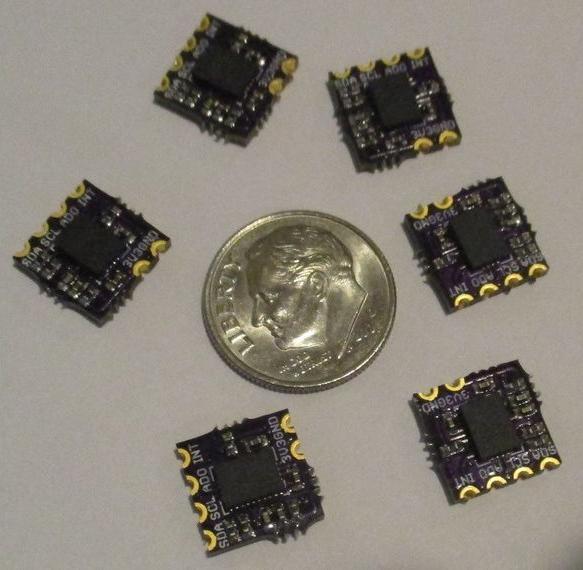
\includegraphics[width=\textwidth]{../common/images/bno055-nano-boards}
                    \imagesource{https://www.tindie.com/products/onehorse/wearable-bno055-nano-board/}
                    \caption{Wearable BNO055 Nano Board}
                \end{figure}
            }
        \end{column}
        \begin{column}{0.6\textwidth}
            \uncover<2->{
                \begin{itemize}
                    \item 32 bit System-in-Package
                    \item tiny ($\SI{10}{mm} \times \SI{10}{mm}$)
                    \item easy to use
                    \item good performance (\textasciitilde{}\SI{100}{Hz})
                \end{itemize}
            }

            \uncover<3->{
                however...
                \begin{itemize}
                    \item ca. \EUR{24} each
                    \item ships from USA
                    \item gyro clipping problems
                \end{itemize}
            }
        \end{column}
    \end{columns}

    \vfill

    \notes{
        \item we had to choose between MPU-9150 and BNO-055
        \item both seemed fit
        \item BNO easier to use
        \item very small board available
        \item but more expensive
    }

    % \footnotetext[1]{\tiny{}\url{https://ae-bst.resource.bosch.com/media/_tech
    % /media/product_flyer/BNO055_Productflyer_BST_20170109.pdf}}
    % https://ae-bst.resource.bosch.com/media/_tech/media/datasheets/BST_BNO055_DS000_14.pdf
\end{frame}

\againframe<1-2>{imus}


\subsection{Microprocessor}

\begin{frame}{Microprocessor}{Adafruit Feather M0 WiFi}
    \begin{columns}[T]
        \begin{column}{0.5\textwidth}
            \uncover<2->{
                \begin{itemize}
                    \item very small and lightweight (6.1g)
                    \item on-board WiFi
                    \item 6 SERCOMs (SPI/I2C/UART)
                \end{itemize}
            }
            \uncover<3->{
                \begin{itemize}
                    \item Arduino\textsuperscript{\textregistered} compatible
                    \item 256KB FLASH, 32KB SRAM
                    \item LiPo charger
                \end{itemize}
            }
            \uncover<4->{
                however...
                \begin{itemize}
                    \item no EEPROM
                    \item ca. \EUR{40} each
                \end{itemize}
            }
        \end{column}

        \begin{column}{0.5\textwidth}
            \uncover<1->{
                \begin{figure}
                    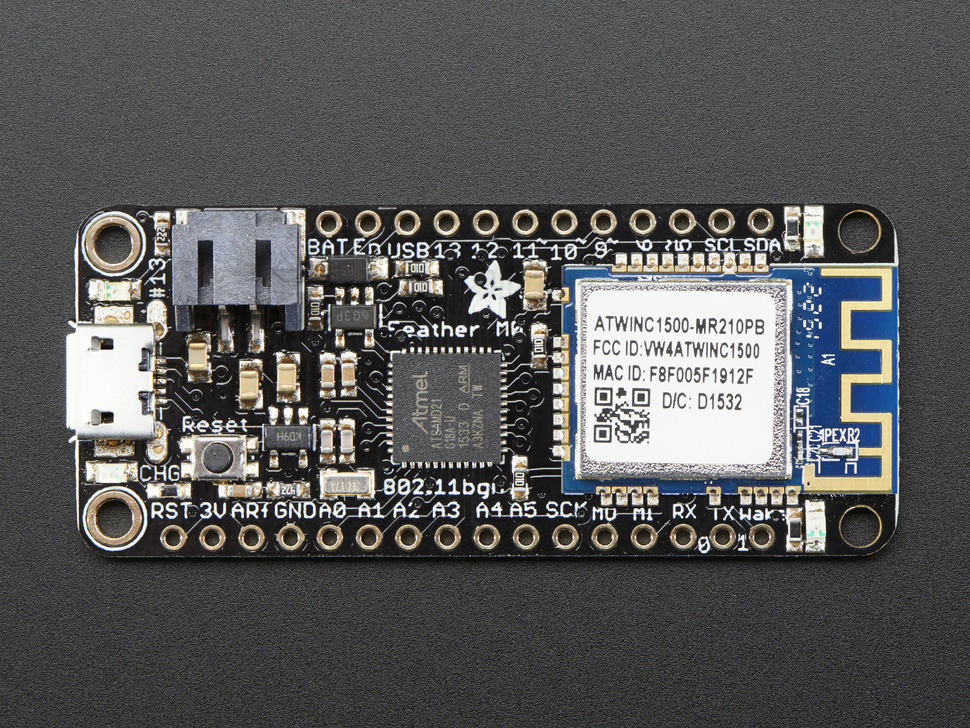
\includegraphics[width=\textwidth]{../common/images/feather-m0-wifi}
                    \imagesource{https://www.adafruit.com/product/3010}
                    \caption{Adafruit Feather M0 WiFi - ATSAMD21 + ATWINC1500 product image}
                \end{figure}
            }
        \end{column}
    \end{columns}

    \notes{
        \item we chose this microprocessor
        \item alternative was Teensy 3.2, but that had some disadvantages
        \item small \& light $\rightarrow$ required for hand-attached device
        \item WiFi $\rightarrow$ no cable that impedes movement
        \item enough SERCOMs
        \item LiPo charger is useful
        \vspace{1em}
        \item we need EEPROM for WiFi credentials $\rightarrow$ so we attached one ourselves
        \item more expensive than Teensy
    }
\end{frame}

\subsection{Architecture}

\begin{frame}<1-2>[label=overview]
    \frametitle<1-2>{Architecture}
    \frametitle<3>{Glove $\leftrightarrow$ PC connection}
    \frametitle<4->{Machine Learning}

    \scalebox{0.7}{
        \begin{tikzpicture}[
    onslide/.code args={<#1>#2}{%
        \ifdefined\only
        \only<#1>{\pgfkeysalso{#2}}%
        \else
        #2
        \fi
    },
    every node/.style={
        font=\small,
        inner sep=0pt,
        thick,
    },
    node distance=2cm,
    database/.style={
        cylinder,
        shape border rotate=90,
        aspect=0.2,
        draw,
        minimum width=2.5cm,
        text width=2.5cm,
        align=center,
        minimum height=1.5cm,
    },
    node/.style={
        rectangle,
        draw,
        text width=2.5cm,
        align=center,
        minimum height=1cm,
        rounded corners=2pt,
    },
    arrow/.style={
        thick,
        ->,
        >=stealth,
    },
    learning/.style={
        dashed,
    },
    applying/.style={
        very thick,
    },
    radiation/.style={
        decorate,
        decoration={expanding waves,angle=10,segment length=4pt}
    },
    wire/.style={
        % draw=gray,
    },
    sensor/.style={
        node,
        minimum width=5mm,
        minimum height=5mm,
        text width=0,
        draw,
        rectangle,
        rounded corners=0,
    },
    highlight/.style={
        draw=primary,
        color=primary,
        fill=primary!10!white,
    },
    drawhighlight/.style={
        thick,
        draw=primary,
    },
    texthighlight/.style={
        color=primary,
    },
]

    \coordinate (legend) at (6.5, 0.2);
    \draw[thick,wire]           ($ (legend) + (0,    0) $) -- node[at end, right, xshift=0.2cm] {Wire}  ++(0.5, 0);
    \draw[thick,arrow,learning] ($ (legend) + (0, -0.6) $) -- node[at end, right, xshift=0.2cm] {Learn} ++(0.5, 0);
    \draw[thick,arrow,applying] ($ (legend) + (0, -1.2) $) -- node[at end, right, xshift=0.2cm] {Apply} ++(0.5, 0);
    \draw ($ (legend) + (-0.2, 0.3) $) rectangle ++(2, -1.8);

    \node[node]
        (serialparser)
        at (0, 0)
        {Serial Parser};

    \node[node,left=2cm of serialparser]
        (sender)
        {Micro-\\processor};

    \node[sensor,below left=7mm and 0.5cm of sender.south]  (sensor1) {};
    \node[sensor,below=2mm of sensor1] (sensor2) {};
    \node[sensor,below=2mm of sensor2] (sensor3) {};
    \node[sensor,below right=7mm and 0.5cm of sender.south] (sensor4) {};
    \node[sensor,below=2mm of sensor4] (sensor5) {};
    \node[sensor,below=2mm of sensor5] (sensor6) {};

    \node[below=3cm of sender] {Sensors};
    \draw[wire,onslide={<2> drawhighlight}] (sensor1) -| ($ (sender.south) + (-0.2, 0) $);
    \draw[wire,onslide={<2> drawhighlight}] (sensor2) -| ($ (sender.south) + (-0.12, 0) $);
    \draw[wire,onslide={<2> drawhighlight}] (sensor3) -| ($ (sender.south) + (-0.04, 0) $);
    \draw[wire,onslide={<2> drawhighlight}] (sensor4) -| ($ (sender.south) + (0.2, 0) $);
    \draw[wire,onslide={<2> drawhighlight}] (sensor5) -| ($ (sender.south) + (0.12, 0) $);
    \draw[wire,onslide={<2> drawhighlight}] (sensor6) -| ($ (sender.south) + (0.04, 0) $);

    \draw[radiation,onslide={<3> drawhighlight}]
        ([xshift=2mm,yshift=-0.3cm]sender.east) -- node[midway,yshift=-0.6cm,onslide={<3> texthighlight}] {or WiFi} ([xshift=-2mm,yshift=-0.3cm]serialparser.west);

    \draw[very thick,wire,onslide={<3> drawhighlight}]
        ([yshift=0.2cm]sender.east) -- node[midway,yshift=0.3cm,onslide={<3> texthighlight}] {USB} ([yshift=0.2cm]serialparser.west);

    \node[node,right=1cm of serialparser]
        (keyboard)
        {Keyboard\\Listener};

    \node[database]
        (bag)
        at ($ (serialparser) + (1.75, -2) $)
        {ROS Bag};

    \node[node,text width=6cm,onslide={<5> highlight}]
        (preprocessing)
        at ($ (serialparser) + (1.75, -4) $)
        {Preprocessing};

    \node[node, below=1cm of preprocessing.south west,anchor=north west,onslide={<5> highlight}]
        (apply)
        {Apply\\Network};

    \node[database, below=1.5cm of preprocessing.south east,anchor=east,onslide={<5> highlight}]
        (model)
        {Saved Model};

    \node[node, right=1cm of preprocessing,onslide={<5> highlight}]
        (sampling)
        {Sampling};

    \node[node, below=1cm of sampling,onslide={<5> highlight}]
        (learning)
        {Learning};

    \node[node, text width=9.5cm]
        (os)
        at ($ (apply) + (3.5, -2) $)
        {Operating System};

    \draw [arrow,applying] ($ (serialparser) + (-0.5,-0.5) $) -- +(0, -3);
    \draw [arrow,learning] ($ (serialparser) + (0,-0.5) $) -- +(0, -1) -- (bag);
    \draw [arrow,learning] ($ (keyboard) + (0,-0.5) $) -- +(0, -1) -- (bag);
    \draw [arrow,learning] (bag) -- (preprocessing);
    \draw [arrow,applying] ($ (preprocessing) + (-2.25,-0.5) $) -- +(0, -1);
    \draw [arrow,applying] (model) -- (apply);
    \draw [arrow,learning] (preprocessing) -- (sampling);
    \draw [arrow,learning] (sampling) -- (learning);
    \draw [arrow,learning] (learning) -- (model);
    \draw [arrow,applying] ($ (apply) + (-0.5,-0.5) $) -- +(0, -1);

    \draw[dotted,line width=2pt] ($ (serialparser) !.5! (sender) + (0, -1.5) $) -- node[at end] (bottom) {} +(0, -8);
    \draw[dotted,line width=2pt] ($ (serialparser) !.5! (sender) + (0, 1) $) -- +(0, 0.5);

    \node[anchor=north west,right=10mm of bottom,yshift=0.5em] {\large{}\textbf{HOST PC}};
    \node[anchor=north east,left=10mm of bottom,yshift=0.5em] {\large{}\textbf{GLOVE}};

    \ifdefined\setbeamertemplate
        \only<1-4>{
            \node[node, anchor=north west, minimum width=9.6cm, minimum height=3.2cm, fill=white] at (preprocessing.north west) {Machine learning};
        }
    \fi
\end{tikzpicture}

    }
\end{frame}

\begin{frame}<1-4>{I2C Bus}{Requirements}
    $$\frac{6\text{ IMUs}}{2\;\frac{\text{addresses}}{\text{IMU}}} = 3\text{ buses}$$

    \pause
    \vspace{1em}

    \begin{table}
    \begin{tabular}{|r||c|c|c|c||c|c|c|c||l|}
        \hline
        & \multicolumn{4}{c||}{Primary pads} & \multicolumn{4}{c|}{Alternative pads} & \\ \hline
        SERCOM
            & 0 & 1 & \color{lightgray}2 & \color{lightgray}3
            & 0 & 1 & \color{lightgray}2 & \color{lightgray}3 & Used by \\ \hline
        0
            & \only<2>{4}
            & 3
            & \color{lightgray}1
            & \color{lightgray}0
            & \only<4>{\cellcolor{primary!25}}A3
            & \only<4>{\cellcolor{primary!25}}A4
            & \color{lightgray}\only<2>{8}
            & \color{lightgray}9
            & Serial1 \\
        1
            & 11
            & 13
            & \color{lightgray}10
            & \color{lightgray}12
            &
            &
            &
            &
            & \\
        2
            & 22
            &
            & \color{lightgray}\only<2>{2}
            & \color{lightgray}5
            & \only<2>{4}
            & 3
            & \color{lightgray}1
            & \color{lightgray}0
            & \\
        3
            & 20
            & 21
            & \color{lightgray}6*
            & \color{lightgray}\only<2>{7*}
            & \only<4>{\cellcolor{primary!25}}11
            & \only<4>{\cellcolor{primary!25}}13
            & \color{lightgray}10
            & \color{lightgray}12
            & Default I2C \\
        4
            & 22
            &
            & \color{lightgray}23*
            & \color{lightgray}24*
            & A1
            & A2
            & \color{lightgray}\only<2>{2}
            & \color{lightgray}5
            & SPI \\
        5
            & A5*
            &
            & \color{lightgray}6
            & \color{lightgray}\only<2>{7}
            & \only<4>{\cellcolor{primary!25}}20
            & \only<4>{\cellcolor{primary!25}}21
            &
            &
            & Debug Port\\
        \hline
    \end{tabular}
    \vspace{2mm}
    {\scriptsize* need to be configured as \emph{SERCOM alt}}
    \caption{Available SERCOM pin pads on Adafruit Feather M0 WiFi}
    \end{table}

    \notes {
        \item these are the available pins for the different SERCOMs on the Feather M0
        \item we need pads 0 und 1 for I2C (fixed)
        \item pins 2, 4, 7, 8 are required for WiFi
        \item so we picked the \textcolor{red}{red marked}
    }
\end{frame}

\begin{frame}[fragile]{I2C Bus}{Arduino Setup}
    \begin{minted}[style=arduino,fontsize=\scriptsize]{c}
#include <Wire.h>
#include <wiring_private.h>

TwoWire wire0(&sercom0, A3, A4);
TwoWire wire1(&sercom3, 11, 13);
TwoWire wire2(&sercom5, 20, 21);

void setup() {
    wire0.begin(); wire0.setClock(400000L);
    wire1.begin(); wire1.setClock(400000L);
    wire2.begin(); wire2.setClock(400000L);
    delay(100);

    pinPeripheral(A3, PIO_SERCOM_ALT); // SERCOM0.0 (alt)
    pinPeripheral(A4, PIO_SERCOM_ALT); // SERCOM0.1 (alt)
    pinPeripheral(11, PIO_SERCOM_ALT); // SERCOM3.0 (alt)
    pinPeripheral(13, PIO_SERCOM_ALT); // SERCOM3.1 (alt)
    pinPeripheral(20, PIO_SERCOM_ALT); // SERCOM5.0 (alt)
    pinPeripheral(21, PIO_SERCOM_ALT); // SERCOM5.1 (alt)
}
    \end{minted}
\end{frame}

\againframe<3>{overview}

\begin{frame}[fragile]{Glove $\leftrightarrow$ PC Connection}{WiFi}
    \begin{columns}[T]
        \begin{column}{0.5\textwidth}
            \begin{minted}[style=arduino,fontsize=\tiny]{c}
// Setup
WiFi.setPins(8, 7, 4, 2);
WiFi.begin();

// Scan for networks (optional)
uint8_t ssidCount = WiFi.scanNetworks();
for (uint8_t i = 0; i < ssidCount; i++) {
    printf("- %s\n", WiFi.SSID(i));
}

// Connect to WPA2 network
uint8_t status = WiFi.begin(MY_SSID, MY_PASSPHRASE);
while (status != WL_CONNECTED) {
    delay(500);
    status = WiFi.status();
}

// Send data via UDP
WiFiUDP wifiUdp;
wifiUdp.begin(8080);
wifiUdp.beginPacket(TARGET_IP, TARGET_PORT);
wifiUdp.write(buffer, length);
wifiUdp.endPacket();
            \end{minted}
        \end{column}
        \begin{column}{0.5\textwidth}
            Capabilities
            \begin{itemize}
                \item WEP \& WPA2
                \item Scan networks
                \item UDP, TCP, SSL
                \item HTTP Client
                \item HTTP Server
            \end{itemize}
        \end{column}
    \end{columns}
\end{frame}


\begin{frame}{System design}{Other Considerations}
    \begin{itemize}
        \item serial protocol for data transmission
        \item attachment to the hand
        \item use ROS for recording \& data analysis
    \end{itemize}
\end{frame}
%
% \subsection{Data Transmission}

% \setbeamercovered{transparent}
% \begin{frame}{Data Transmission}{Protocol Requirements}
%     \centering
%     \vfill\null
%     \def\arraystretch{1.5}
%     \scriptsize
%     \begin{tabular}{p{0.45\textwidth}|p{0.45\textwidth}}
%         \textbf{Requirement} & \textbf{Means} \\ \hline\hline
%         fast $\rightarrow$ lightweight & self made solution \pause \\
%         supports USB \& WiFi & package based protocol \pause \\
%         simple to write \& parse & simple buffer layout \pause \\
%         robust & package start/end checks \pause \\
%         flexible & versioned \pause \\
%         time critical & timestamps included in every message \pause \\
%         metadata: imu count, sensibility & header packet
%     \end{tabular}
%     \vfill\null
% \end{frame}
% \setbeamercovered{invisible}

